\documentclass[sigconf]{acmart}

\usepackage{algorithmic}
\usepackage{algorithm}
\usepackage{hyperref}
\usepackage{bbold}
\usepackage{enumitem}
\usepackage{graphicx}
\usepackage{bm}
\usepackage[newfloat,cache=false]{minted}

\begin{document}

\title{COMP6247 - Kalman Filter}
\author{Luke McClure \\ lam3g17@soton.ac.uk \\ 29573904}

\maketitle

\pagestyle{myheadings} 
\section{Background}
Kalman Filter is a method to estimate the parameters of a time series model in an online fashion. This is completed by estimating the parameters $\theta$ and covariance $P$ and updating these as new information is revealed.
\begin{align}
  \boldsymbol{\theta}(n|n-1) = \boldsymbol{\theta}(n-1|n-1) \\
  P(n|n-1) = P(n-1|n-1) + Q
  \label{eqn:p}
\end{align}
\begin{align}
  \boldsymbol{\theta}(n|n) = \boldsymbol{\theta}(n|n-1) + \boldsymbol{k}(n)e(n) \\
  P(n|n) = (\mathcal{I} - \boldsymbol{k}(n)\boldsymbol{x}(n)^{T})P(n|n-1)
  \label{eqn:thet}
\end{align}
\begin{equation}
  \boldsymbol{k}(n) = \frac{P(n|n-1)\boldsymbol{x}(n)}{R + \boldsymbol{x}(n)^{T}P(n|n-1)\boldsymbol{x}(n)}
  \label{eqn:k}
\end{equation}
\section{Convergence over different initial conditions}
By standardising $A$, $R$, and $Q$, we can investigate how different random initial values of $\theta$ converge when using Kalman filtering. This allows us to build a general picture of how well Kalman filtering performs on a general series using these hyperparameters. 

%% easy change to reduce space - set this to 5 piece table and set width = 100mm
\begin{figure}[h]
  \centering
    \begin{tabular}{c}
    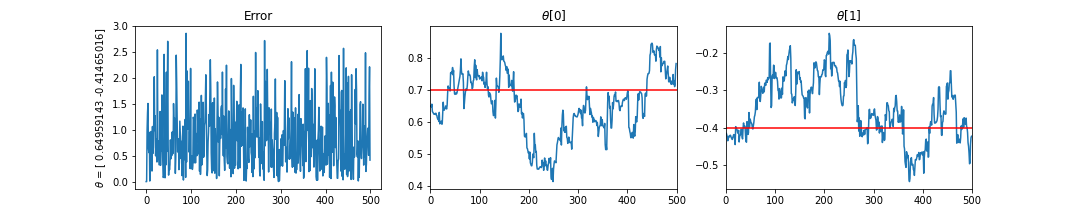
\includegraphics[width=120mm]{"../&theta-0.png"} \\
    (a) $\theta = [0.65, -0.41]$ \\[6pt]
    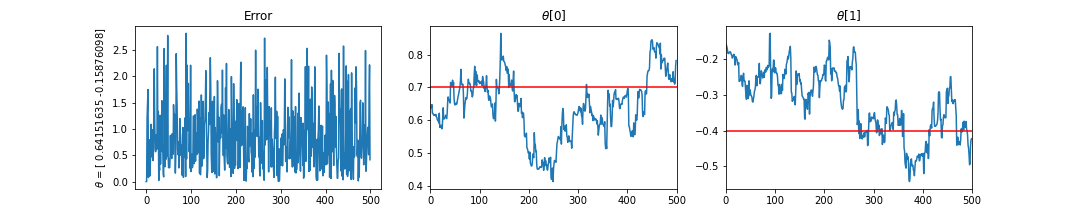
\includegraphics[width=120mm]{"../&theta-1.png"} \\
    (b) $\theta = [0.64, -0.16]$ \\[6pt]
     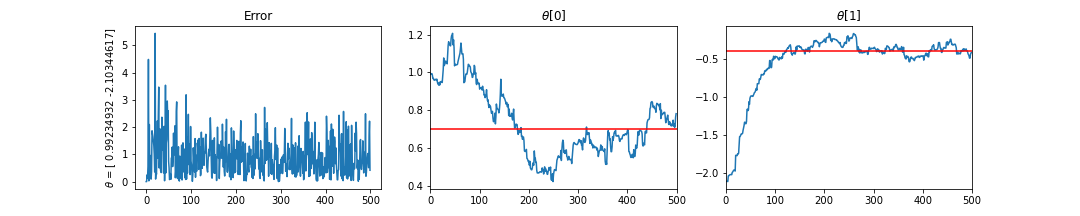
\includegraphics[width=120mm]{"../&theta-2.png"} \\ 
    (c) $\theta = [ 0.99, -2.10]$ \\[6pt]
    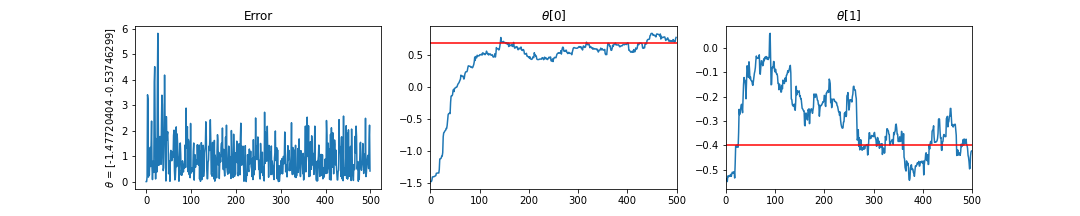
\includegraphics[width=120mm]{"../&theta-3.png"} \\
    (d) $\theta = [-1.48, -0.54]$ \\[6pt]
    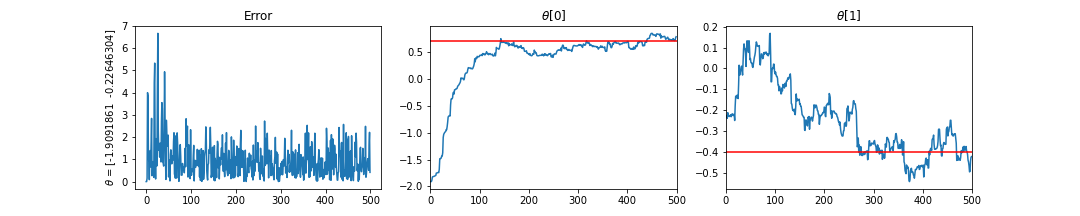
\includegraphics[width=120mm]{"../&theta-4.png"} \\
    (e) $\theta = [-1.91, -0.23]$ \\[6pt]
    \end{tabular}
    \caption{Varying initial starting conditions $\theta $ with $A = [0.7, -0.4], R = 0.2\sigma(S_{A}), Q = 0.0001\mathcal{I}  $}
    \label{fig:initconditions}
  \end{figure}

Over all samples shown in \autoref{fig:initconditions}, Kalman Filter was able to converge $\theta$ within 50 samples, or was already close to $A$ by chance. This is fairly independent of how far the initial value of $\theta$ was from $A$ suggesting that the gradient of convergence tends to get steeper with a larger difference between the two values. This makes sense as a larger difference between the values of $A$ and $\theta$ results in larger updates being applied (due to a larger prediction error).\\ 

In samples a and b there is less of a convergence pattern as the error stays focused between 0.5 and 1.5. The starting parameters of $\theta$ in these instances were very close to $A$, so it acted as if the filter had already converged. Samples c, d and e show the classic convergence pattern with error starting high (5-7) and dropping very quickly within 50 samples to between 0 and 2. \\

It is interesting to note that in all the plots of $\theta$[0] and $\theta$[1] you can see similar patterns as the filters independently react to the same key features within the original AR series and are "surprised" by them.\\

Even when the error takes only about 50 samples to converge, it takes much longer for $\theta$. In samples c, d and e the components of $\theta$ typically take at least 100 iterations to reach close to their respective component of $A$.
With components of $\theta$ that start closer to their target of $A$, the plot of their change is a lot more noisy. Smaller variations show clearer within these plots and $\theta$ reacts seemingly more strongly to the key features of $S$ that are being encountered by the filters on that iteration. \\

\section{Effects of hyperparameters on convergence}
In \autoref{fig:hyperparam} the left column shows the effects of varying the signal noise variance $R$, and the right shows the effects of varying the process noise covariance $Q$. 
Both variations take the initial parameters from \autoref{fig:initconditions} and vary the order of magnitude +/- 1. In both cases the other variable is left at the same value from \autoref{fig:initconditions} and both $A$ and $\theta$ are left constant. The same AR series S has been used over all experiments within this section.
\begin{figure}[h]
  \centering
    \begin{tabular}{cc}
    \hline   
        Varying R ($Q = 0.0001\mathcal{I}$) & Varying Q ($R = 0.1\sigma(S_{A})$) \\
    \hline
      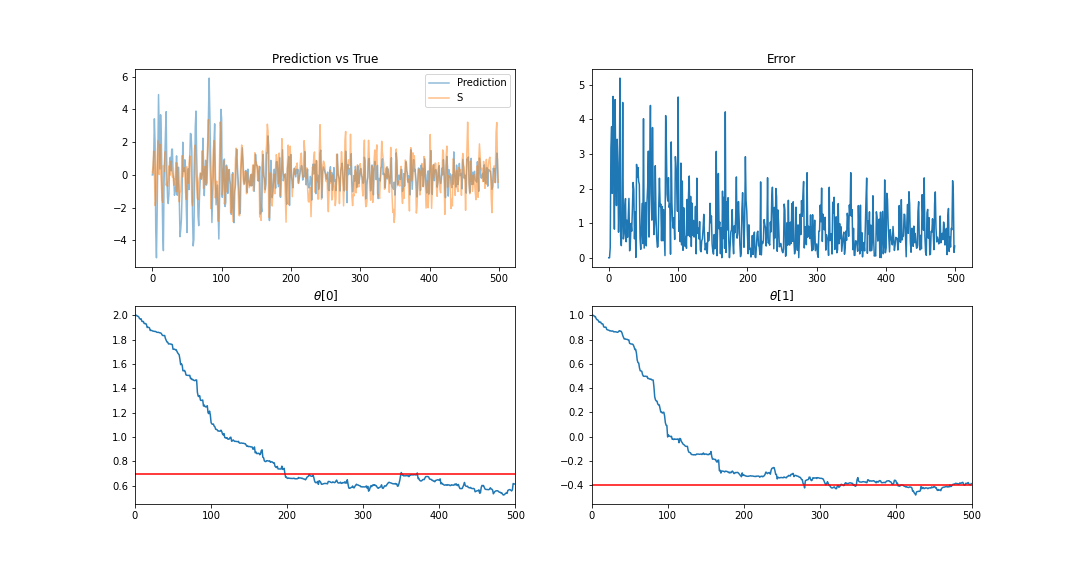
\includegraphics[width=80mm]{"../R-1.png"} &   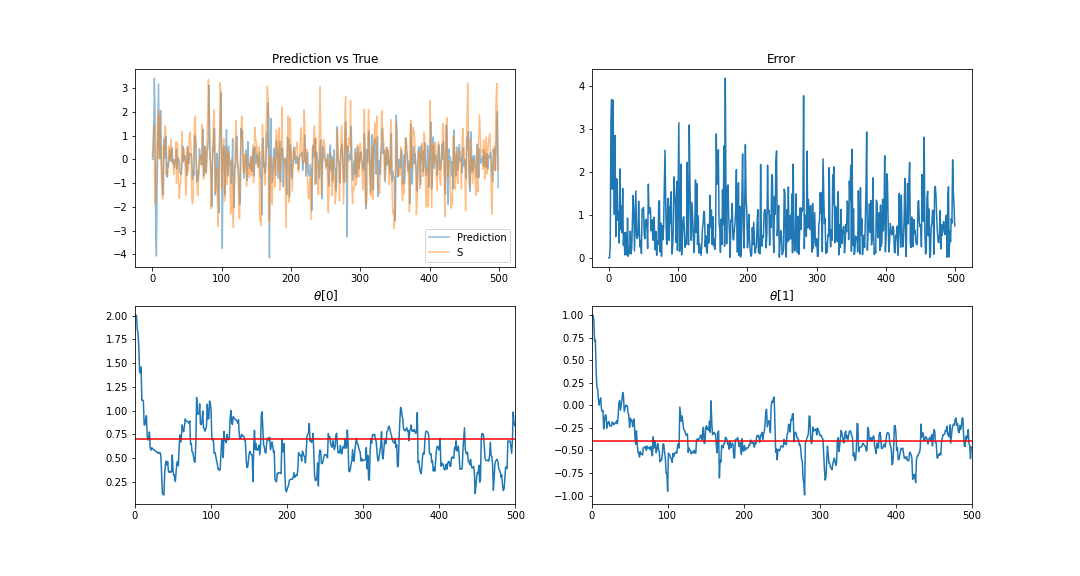
\includegraphics[width=80mm]{"../Q-0.001.png"} \\
    (a) $R = \sigma(S_{A})$ & (b) $Q = 0.001\mathcal{I}$\\[6pt]
     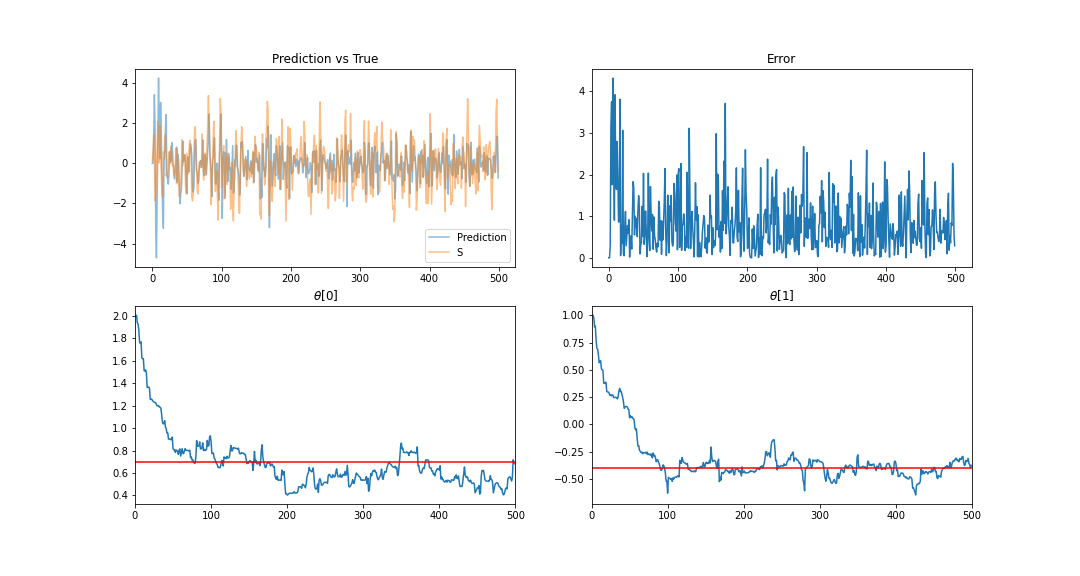
\includegraphics[width=80mm]{"../R-0.1.png"} &   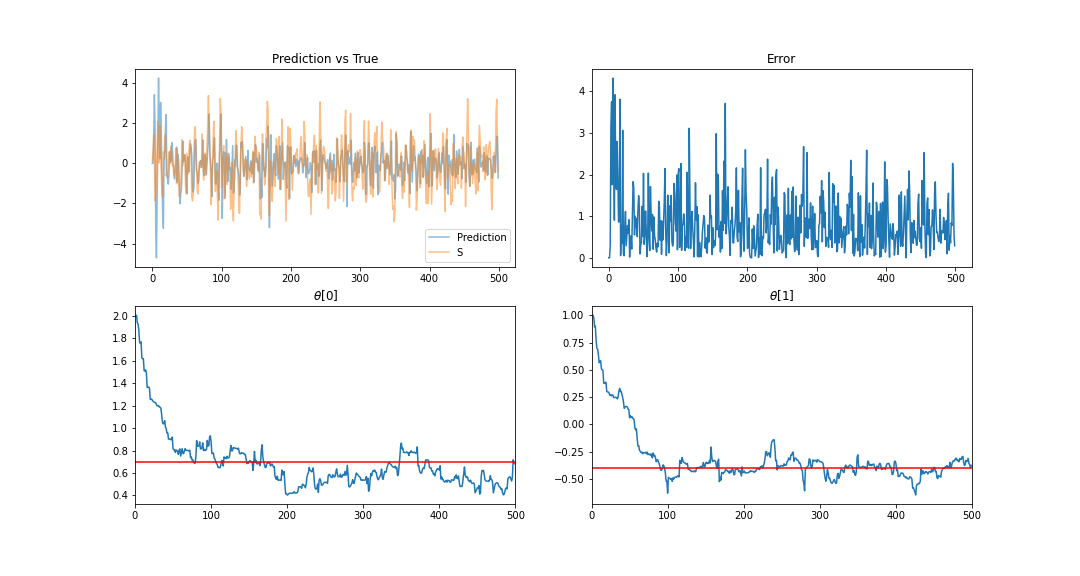
\includegraphics[width=80mm]{"../Q-0.0001.png"} \\
    (c) $R = 0.1\sigma(S_{A})$ & (d) $Q = 0.0001\mathcal{I}$\\[6pt]
    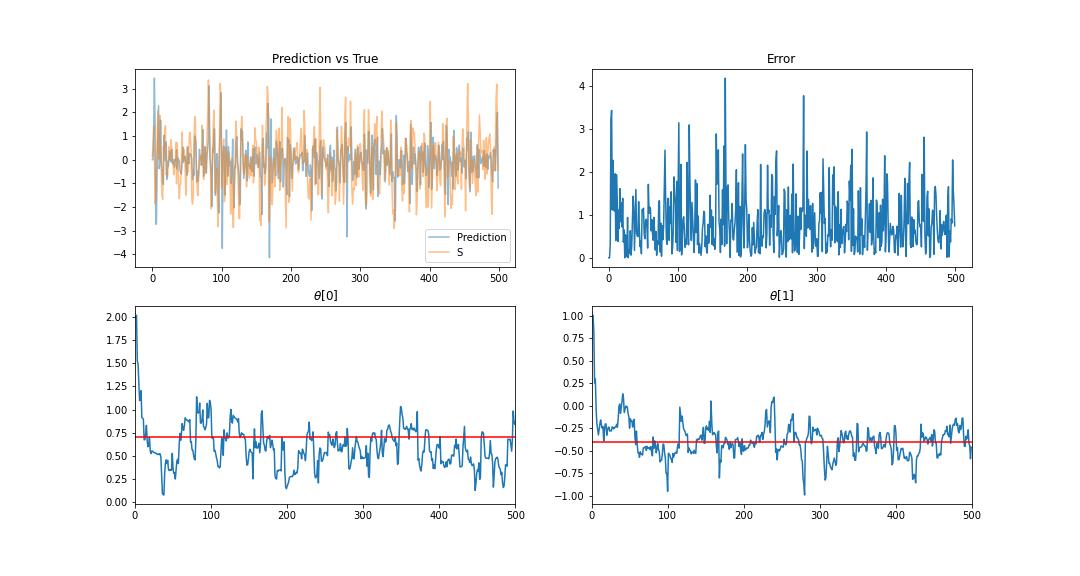
\includegraphics[width=80mm]{"../R-0.01.png"} &   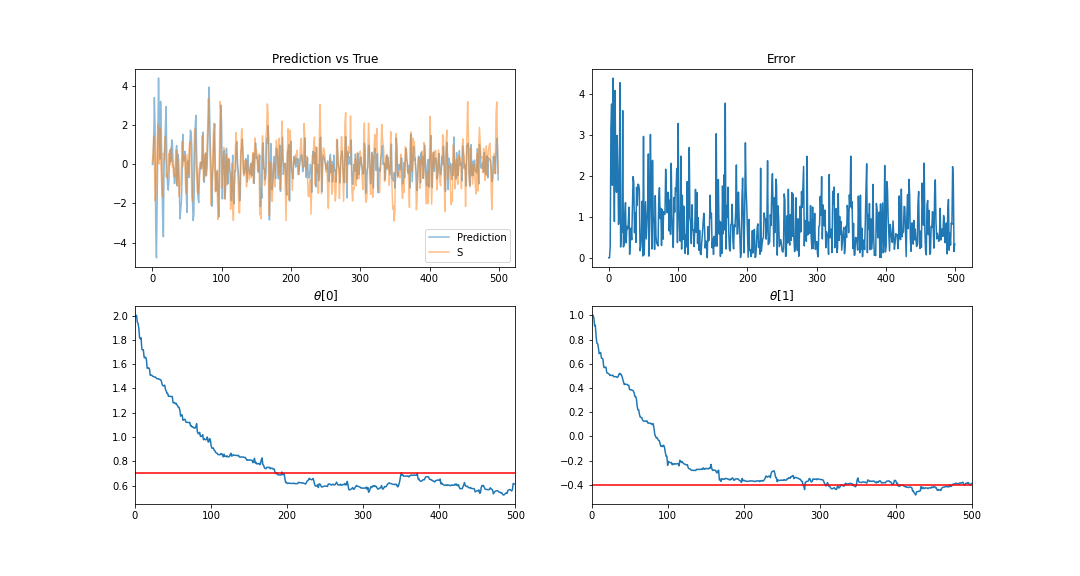
\includegraphics[width=80mm]{"../Q-0.00001.png"} \\
    (e) $R = 0.01\sigma(S_{A})$ & (f) $Q = 0.00001\mathcal{I}$\\[6pt]
    \end{tabular}
    \caption{Varying hyper parameters with $A = [0.7, -0.4], \theta = [2.0, 1.0]$}
    \label{fig:hyperparam}
\end{figure}
\subsection{Varying signal noise variance $R$}
Signal noise covariance is the amount of noise from the measurement of the signal. Convergence speed is inversely proportional to the magnitude of $R$ from this data, with experiment a taking around 100 samples to converge whilst experiment e converging almost instantly.
There seems to be a slight stability correlation with the magnitude of $R$ as well, with experiment a seeming to settle much more than experiment e when it has finally converged.\\

Looking at $\theta$ it is easy to confirm all of the hypotheses from the trend of error across experiments a, c and e.
It is clear how $\theta$ takes much longer to converge in experiment a than in e, showing that $R$ is inversely proportional to convergence speed.
These plots also show how stability of $\theta$ is proportional to $R$, experiment e shows a very volatile search in the neighbourhood of $A$ while in both experiments c and a when $\theta$ eventually converges on $A$ it stays relatively close.\\

This makes sense when thinking about the role $R$ has to play within Kalman Filtering. An increase of $R$ indicates that the system should not trust the data as much, and so must take longer to eventually converge. This can be seen clearly in \autoref{eqn:k} where $R$ only appears in the denominator.
The inverse relationship with stability is also a result of the inverse nature of $R$ and $k(n)$, with a larger $R$ resulting in smaller updates to $\theta$. Settling on the parameters within $\theta$ over a longer time results in every sample not having such a pronounced impact, leading to more stability.
\subsection{Varying process noise covariance $Q$} 
Process noise covariance is a measure of the noise within the signal itself, as $Q$ gets smaller it takes longer for KF to converge on $A$ but this convergence is more stable.\\

Varying process noise covariance has a similar but opposite effect from signal noise variance, there is a proportional relationship between $Q$ and convergence speed.
In this case the convergence is less pronounced in the error function compared to signal noise covariance, the only clear definition of lack of convergence in the error plots are the thicker portions at the immediate start of the plot. All of these non-converged sections end by 50 iterations, but they appear longer with a smaller $Q$.\\

Speed of $\theta$ convergence is proportional to $Q$. The relationship between convergence speed vs stability has the same opposing nature in both $R$ and $Q$, where as the convergence speed decreases the eventual convergence is more stable or vice versa. \\

\begin{figure}[H]
  \centering
\begin{tabular}{ c c c }
  Hyperparameter & Error & Stability \\
  \hline
  \hline
  R & Inversely proportional & Proportional \\
  Q & Proportional & Inversely proportional \\
\end{tabular}
\caption{Summary of hyperparameters proportionality with convergence speed}
\end{figure}
\section{Constant vs Time Varying AR processes}
Kalman filtering works not only with stationary AR's, but also time varying AR's where the parameters $A$ shift with time according to defined functions.

To investigate the KF on both these, I used the same values for $A$ to generate a stationary AR, and as $a$ in a time varying AR with \autoref{eqn:tvar}. The only difference between each output from the same category is the randomly generated excitation.

\begin{align}
  A[0] = a[0] + \cos(2 * \pi * n) \\
  A[1] = a[1] + 1.4 * \sin(6 * \pi * n) 
  \label{eqn:tvar}
\end{align}

Looking at \autoref{fig:TVAR}, KF is able to adapt and converge to the time varying AR as fast as the stationary AR.\\
Within experiment b the Kalman Filter quickly picks up of the underlying function in $\theta$[1] but struggles to fully match the function in $\theta$[0], although there appears to be a hint of the cosine wave within $\theta$[0] albeit slightly lagged behind the $A$[0].
The $\theta$ convergences seem to be slightly faster in the experiment b too but this is up for interpretation in $\theta$[0], $\theta$[0] is matched much better in experiment a. 
\begin{figure}[h]
  \centering

    \begin{tabular}{cc}
      \hline
      Constant A & Time Varying A \\
      \hline 
    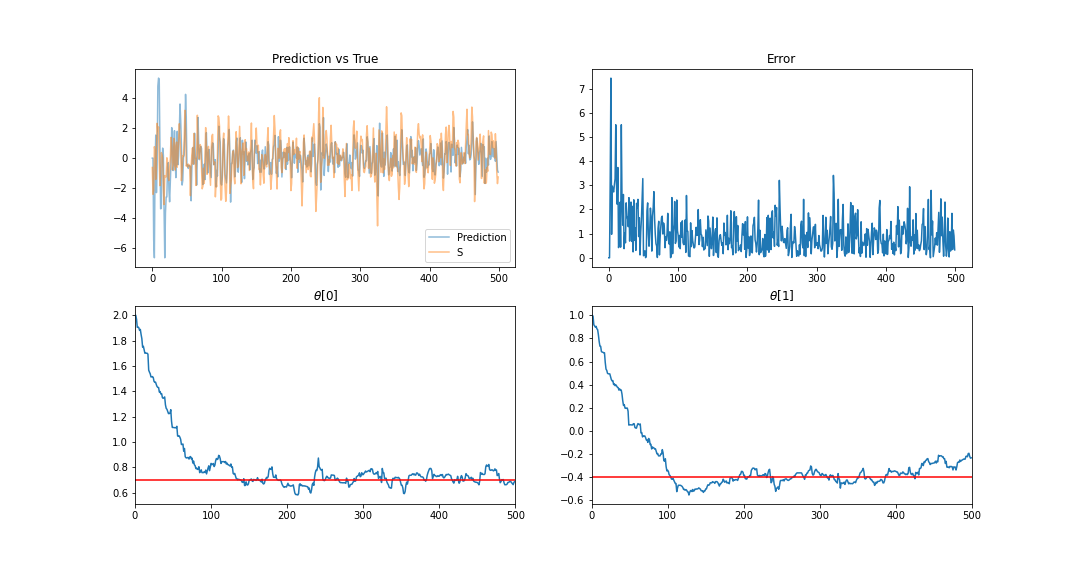
\includegraphics[width=80mm]{"../T-TS.png"} & 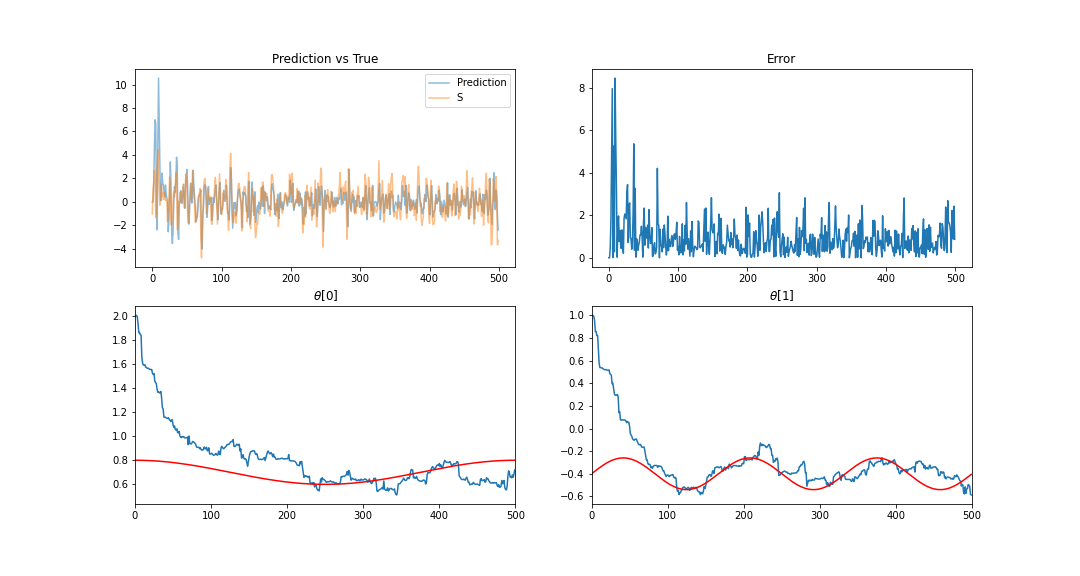
\includegraphics[width=80mm]{"../T-TV.png"} \\
    (a) Constant A - 1 & (b)  Time Varying A - 1\\[6pt]
    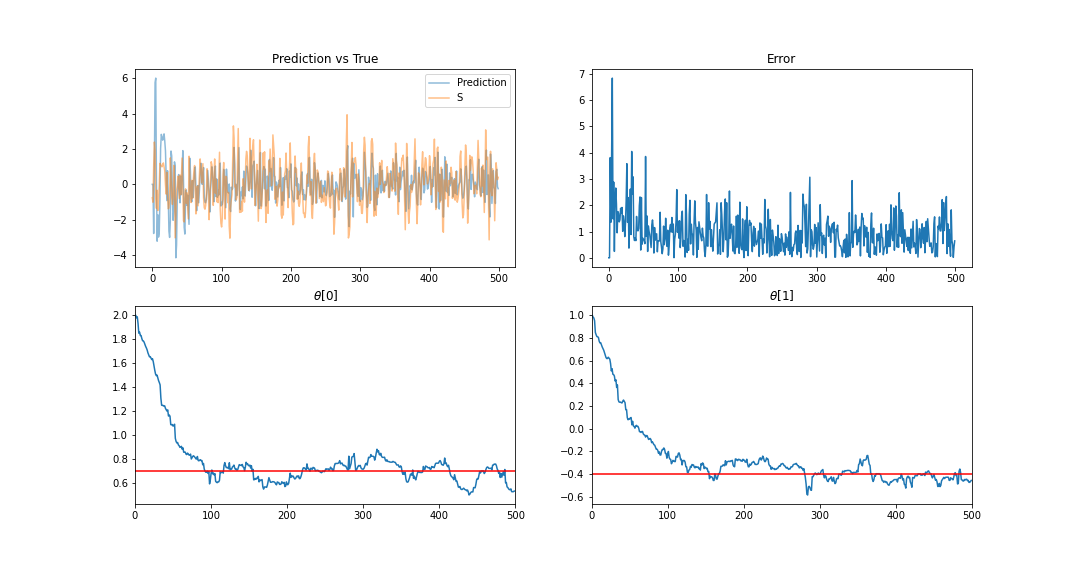
\includegraphics[width=80mm]{"../T-TS2.png"} & 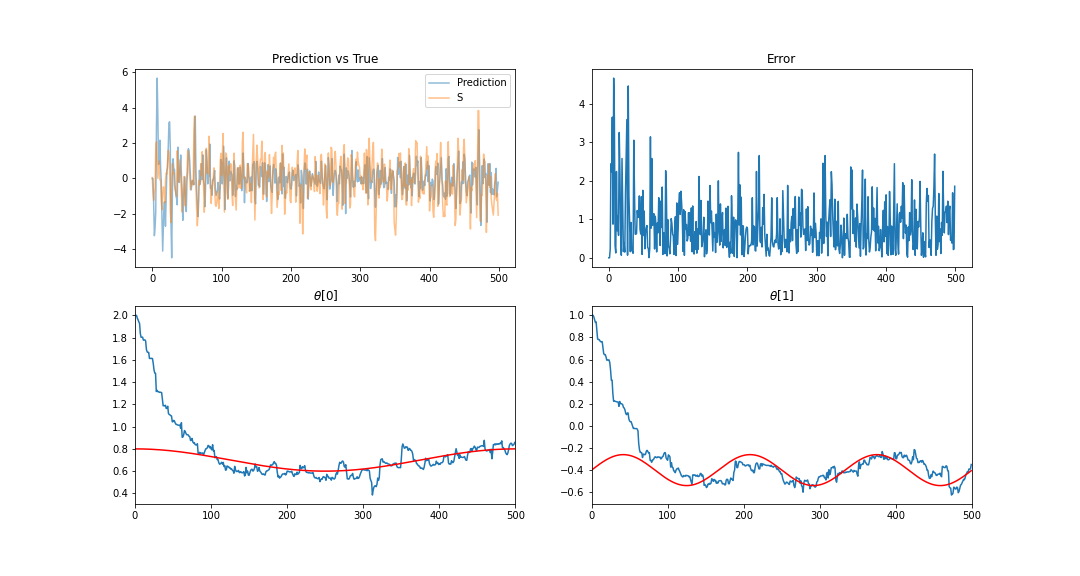
\includegraphics[width=80mm]{"../T-TV2.png"} \\
    (c) Constant A - 2 & (d)  Time Varying A - 2 \\[6pt]
    \end{tabular}
    \caption{Varying Constant and Time Varying A with $a = [0.7, -0.4], \theta = [2.0, 1.0], R = 0.2\sigma(S_{A}), Q = 0.0001\mathcal{I}$}
    \label{fig:TVAR}
\end{figure}

Experiment d shows a lot more accurate matching of the time varying components by $\theta$, with the periodic functions reflected between iterations 100-200 and by iteration 300 both components of $\theta$ have almost matched their counterparts in $A$.
\end{document}
\endinput